\documentclass[a4paper,11.5pt]{article}
\usepackage[textwidth=170mm, textheight=230mm, inner=20mm, top=20mm, bottom=30mm]{geometry}
\usepackage[normalem]{ulem}
\usepackage[utf8]{inputenc}
\usepackage[T1]{fontenc}
\PassOptionsToPackage{defaults=hu-min}{magyar.ldf}
\usepackage[magyar]{babel}
\usepackage{amsmath, amsthm,amssymb,paralist,array, ellipsis, graphicx, float}
%\usepackage{marvosym}

\makeatletter
\renewcommand*{\mathellipsis}{%
	\mathinner{%
		\kern\ellipsisbeforegap%
		{\ldotp}\kern\ellipsisgap%
		{\ldotp}\kern\ellipsisgap%
		{\ldotp}\kern\ellipsisaftergap%
	}%
}
\renewcommand*{\dotsb@}{%
	\mathinner{%
		\kern\ellipsisbeforegap%
		{\cdotp}\kern\ellipsisgap%
		{\cdotp}\kern\ellipsisgap%
		{\cdotp}\kern\ellipsisaftergap%
	}%
}
\renewcommand*{\@cdots}{%
	\mathinner{%
		\kern\ellipsisbeforegap%
		{\cdotp}\kern\ellipsisgap%
		{\cdotp}\kern\ellipsisgap%
		{\cdotp}\kern\ellipsisaftergap%
	}%
}
\renewcommand*{\ellipsis@default}{%
	\ellipsis@before
	\kern\ellipsisbeforegap
	.\kern\ellipsisgap
	.\kern\ellipsisgap
	.\kern\ellipsisgap
	\ellipsis@after\relax}
\renewcommand*{\ellipsis@centered}{%
	\ellipsis@before
	\kern\ellipsisbeforegap
	.\kern\ellipsisgap
	.\kern\ellipsisgap
	.\kern\ellipsisaftergap
	\ellipsis@after\relax}
\AtBeginDocument{%
	\DeclareRobustCommand*{\dots}{%
		\ifmmode\@xp\mdots@\else\@xp\textellipsis\fi}}
\def\ellipsisgap{.1em}
\def\ellipsisbeforegap{.05em}
\def\ellipsisaftergap{.05em}
\makeatother

\usepackage{hyperref}
\hypersetup{
	colorlinks = true	
}
\DeclareMathOperator{\Int}{int}
\DeclareMathOperator{\tg}{tg}
\DeclareMathOperator{\ctg}{ctg}
\DeclareMathOperator{\Th}{th}
\DeclareMathOperator{\sh}{sh}
\DeclareMathOperator{\ch}{ch}
\DeclareMathOperator{\arc}{arc}
\DeclareMathOperator{\arctg}{arc tg}
\DeclareMathOperator{\arcctg}{arc ctg}

\begin{document}
	%%%%%%%%%%%RÖVIDÍTÉSEK%%%%%%%%%%
	\setlength\parindent{0pt}
	\def\s{\hspace{0.2mm}\vphantom{\beta}}
	\def\Z{\mathbb{Z}}
	\def\Q{\mathbb{Q}}
	\def\R{\mathbb{R}}
	\def\C{\mathbb{C}}
	\def\N{\mathbb{N}}
	\def\Rn{\mathbb{R}^{n}}
	\def\Ra{\overline{\mathbb{R}}}
	\def\sume{\displaystyle\sum_{n=1}^{+\infty}}
	\def\sumn{\displaystyle\sum_{n=0}^{+\infty}}
	\def\biz{\emph{Bizonyítás:\ }}
	\def\narrow{\underset{n\rightarrow+\infty}{\longrightarrow}}
	\def\limn{\displaystyle\lim_{n\to +\infty}}
	\def\limx{\displaystyle\lim_{x\to +\infty}}
	
	\theoremstyle{definition}
	\newtheorem{theorem}{Tétel}[subsection] % reset theorem numbering for each chapter
	
	\theoremstyle{definition}
	\newtheorem{definition}[theorem]{Definíció} % definition numbers are dependent on theorem numbers
	\newtheorem{example}[theorem]{Példa} % same for example numbers
	\newtheorem{task}[theorem]{Feladat} % same for example numbers
	\newtheorem{note}[theorem]{Megjegyzés} % same for example numbers
	\newtheorem{revision}[theorem]{Emlékeztető} % same for example numbers
	%%%%%%%%%%%%%%%%%%%%%%%%%%%%%%%%%
	\begin{center}
		{\LARGE \textbf{Analízis II.}}
		
		{\large \textbf{Gyakorlati óra jegyzet}}
		
		11. óra
	\end{center}
	A jegyzetet \textsc{Umann} Kristóf készítette Dr. \textsc{Szili} László gyakorlatán. (\today)
	
	Tantárgyi honlap: \url{http://numanal.inf.elte.hu/~szili/Oktatas/An2_BSc_2016/index_An2_2016.htm}
	\section{Információk}
	\begin{compactitem}
		\item Nem lesz több $+/-$.
		\item Felkerültek a második zh-val kapcsolatos információk.
		\item Felkerültek a bizonyítással kért tételek listája.
		\item Ebből 2 olyan, ami csak hétfőn hangzik el.
		\item Nehezebb feladatok vannak a tematikában, mint ami várható a zh-ban.
	\end{compactitem}
	\section{L'Hospital szabály (folyt.)}
	Ha valahol egy q betű van, aminek nincs ott keresnivalója, szólj! Variáltam a makrókon, és várhatóan be fogom nézni egy párszor.
	\begin{task}
		\[ \lim_{x\to1}\frac{x^2-1}{2x^2-x-1} \quad \overset{\frac{0}{0}}{=}  \quad \lim_{x\to1}\frac{2x}{4x-1}=\frac{2}{3} \]
	\end{task}
	\begin{task}
		\[\lim_{x\to0} \frac{a\tg x-x}{x-\sin x}\quad \overset{\frac{0}{0}}{=}\quad \lim_{x\to0} \frac{\frac{1}{\cos^2x}-1}{1-\cos x}\quad \overset{\frac{0}{0}}{=}\quad \lim_{x\to0}\frac{1-\cos^2 x}{1-\cos x}=\lim_{x\to0}\frac{1+\cos x}{\cos^2x}=\frac{2}{1} \]
		%TODO \cos^2x, nem \frac{2}{x}
		Fejben meggondoltuk, hogy valóban alkalmazható-e a szabály. (deriválható-e egyáltalán a fv.)
	\end{task}
	\begin{task}
		\[\lim_{x\to+\infty}\frac{x^n}{e^x}\quad =\overset{\text{$n$-szer alkalmazzuk a L'Hospital-t}}{\dots}=\quad \lim_{x\to+\infty}\frac{n!}{e^x}=0 \]
	\end{task}
	\begin{note}
		$x^n<<e^x (\text{\quad ha $x$ ,,nagy''})$
	\end{note}
	\begin{task}
		\[ \lim_{x\to1-0}\ln x\cdot\ln(1-x)\quad \overset{0\cdot(-\infty)}{=}\quad \lim_{x\to1-0}\frac{\ln(1-x)}{\frac{1}{\ln x}}\quad \overset{\frac{-\infty}{-\infty}}{=}\quad \lim_{x\to1-0}\frac{\frac{1}{1-x}\cdot(-1)}{-\frac{1}{\ln^2x}\cdot\frac{1}{x}}=\lim_{x\to1-0}\frac{x}{1-x}\cdot\ln^2x=\]
		\[=\lim_{x\to1-0}x\cdot\frac{\ln^2x}{1-x}\quad \overset{\frac{0}{0}}{=}\quad \lim_{x\to1-0}\frac{2\ln x\cdot\frac{1}{x}}{-1}=0. \]
	\end{task}
	\begin{note}
		\begin{figure}[H]
			\centering
			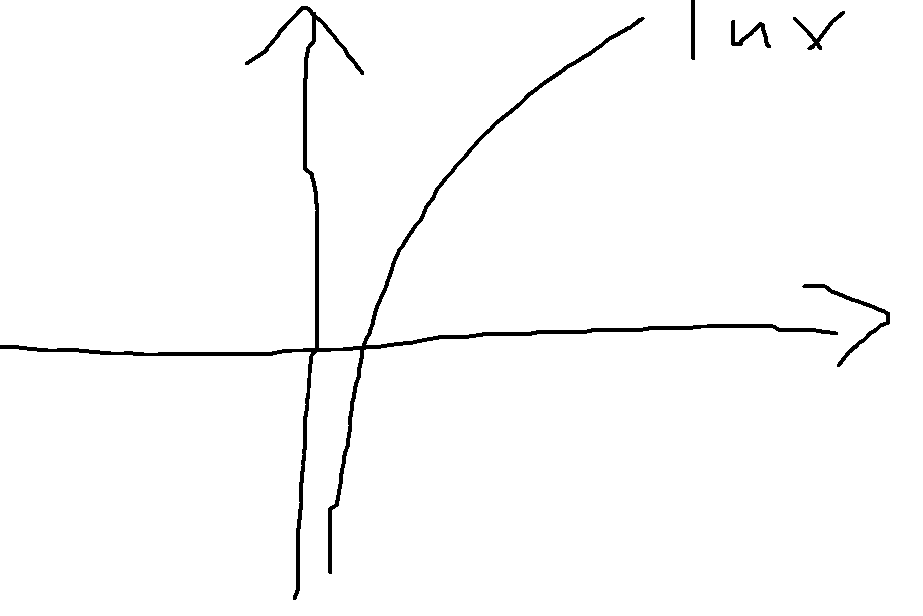
\includegraphics[height=3cm]{kepek/first.png}
			\caption{Figyeljük meg az $\ln$ függvényt. Ezért tehetjük meg a törtté alakítást.}\label{}
		\end{figure}
	\end{note}
	\begin{task}
		\[ \lim_{x\to0}\left(\frac{1}{x}-\frac{1}{e^x-1}\right)=\lim_{x\to0}\frac{e^x-1-x}{x(e^x-1)}\quad \overset{\frac{0}{0}}{=}\quad \lim_{x\to0}\frac{e^x-1}{e^x-1+xe^x}\quad \overset{\frac{0}{0}}{=}\quad \lim_{x\to0}\frac{e^x}{e^x+e^x+xe^x}=\frac{1}{1+1+1\cdot0} \]
	\end{task}
	\begin{task}
		\[ \lim_{x\to+\infty}\left(\frac{2x-3}{2x-5}\right)^{2x+1}\quad \overset{1^{+\infty}}{=}\quad \left(\frac{2x-3}{2x+5}\right)^{2x+1}\quad \overset{a=e^{\ln a}}{=}\quad \left(e^{\ln\frac{2x-3}{2x+5}}\right)^{2x+1}=e^{(2x+1)\ln\frac{2x-3}{2x+5}}=\]
		\[=\lim_{x\to+\infty}(2x+1)\ln\frac{2x-3}{2x+5}=\quad \overset{(+\infty)\cdot0}{=}\quad \lim_{x\to+\infty}\frac{\ln\frac{2x-3}{2x+5}}{\frac{1}{2x+1}}\quad \overset{\frac{0}{0}}{=}\quad \lim_{x\to+\infty}\frac{\displaystyle \frac{1}{\frac{2x-3}{2x+5}}\cdot\frac{2(2x+5)-(2x-3)\cdot2}{(2x+5)^2}}{\displaystyle -\frac{1}{(2x+1)^2}\cdot2} =\]
		\[ =\lim_{x\to+\infty}-\frac{(2x+1)^2}{2}\cdot\frac{16}{(2x-3)(2x+5)}=-\frac{16}{2}\lim_{x\to+\infty}\frac{\left(2+\frac{1}{x}\right)^2}{\left(2-\frac{3}{x}\right)\left(2+\frac{5}{x}\right)}=-8\cdot\frac{4}{4}=-8 \]
	\end{task}
	\section{Taylor-polinomok}
	\begin{task}
		\[ |f(x)-T_{n,a}(f,x)|\leq ? \]
		$f(x):=e^x, (x\in(0,1)); a=0; n\in\N$.
		\begin{revision}
			\[ f\in D\{a\} \Rightarrow f(x)-f(a)=f'(a)(x-a)+\varepsilon(x)(x-a) \]
			Azaz $f(x)$-et lehet közelíteni $f(a)+f'(x)(x-a)$-val.
		\end{revision}
		\textit{Megoldás:}
		
		\[ T_{n,a}(f,x)=\sum_{k=0}^n\frac{f^{(k)}(a)}{k!}(x-a)^k=f(a)+\frac{f'(a)}{1!}(x-a)+\frac{f''(a)}{2!}(x-a)^2+\ldots+\frac{f^{n}(a)}{n!}(x-a)^n \]
		\begin{note}
			Ha magát a Taylor sorösszegét szeretnénk kiszámolni, bajba lennénk a deriválások miatt. $f^{(k)}(a)$ kiszámolása általában nem épp triviális feladat.
			\begin{center}
				\textit{,,De mi nem általában fogunk ZH-t írni, hanem konkrétan!''}
				\smallskip
				
				/Szili László/
			\end{center}
		\end{note}
		\[ f^{(n)}(x)=e^x\quad  \Rightarrow \quad f^{(n)}(0)=1  \]
		\[ T_{n,0}(\exp, x)=\sum_{k=0}^n\frac{f^{(n)}(0)}{k!}x^k=\sum_{k=0}^n\frac{x^k}{k!} \]
		Még egy dologra vagyunk kíváncsiak.
		\[ e^x-T_{n,0}(\exp,x)=e^x-\sum_{k=0}^n\frac{x^k}{k!}\quad \overset{!}{=}\quad \frac{\exp^{(n+1)}(\xi)}{(n+1)!}x^{n+1} \quad \Rightarrow\quad |x|\leq1 \]
		$\exists \xi\in(0,x)\subset(0,1),$
		\[ \left|e^x-\left(1+x\frac{x^2}{2!}+\ldots+\frac{x^n}{n!}\right)\right|=\left|\frac{e^\xi}{(n+1)!}\cdot x^{n+1}\right|\quad \overset{|x|\leq1}{\underset{0<\xi<1}{\leq}}\quad e^1\cdot\frac{1}{(n+1)!}.\quad \blacksquare \]
	\end{task}
	\begin{task}
		\[ f(x):=\sqrt{1+x} (x>-1),\quad |f(x)-T_{n,a}(f,x)|\leq? \]
		$a=0;\quad  n=2;\quad (x\in[0,1])$
		
		\textit{Megoldás:}
		
		\[ T_{2,0}(f;x)=f(0)+\frac{f'(0)}{1!}x+\frac{f''(0)}{2!}x^2 \]
		\[ f(x)=\sqrt{1+x}=(1+x)^{\frac{1}{2}};\quad f(0)=1 \]
		\[ f'(x)=\frac{1}{2}(1+x)^{-\frac{1}{2}};\quad f'(0)=\frac{1}{2} \]
		\[ f''(x)=-\frac{1}{4}(1+x)^{-\frac{3}{2}};\quad f''(0)=-\frac{1}{4} \]
		\[ f'''(x)=\frac{3}{8}(1+x)^{-\frac{5}{2}};\quad f''(0)=-\frac{1}{4} \]
		\[ T_{2,0}(f;x)=1+\frac{\frac{1}{2}}{1!}x+\frac{-\frac{1}{4}}{2!}x^2=1+\frac{x}{2}-\frac{x^2}{8} \]
		\[ x\in[0,1] \quad \overset{\text{Taylor-Lagrange}}{\Longrightarrow}\quad \exists0<\xi<x\leq1 \]
		\[ \left|\sqrt{1-x}-\left(1+\frac{x}{2}-\frac{x^2}{8}\right)\right|= \left|\left(\frac{f'''(\xi)}{3!}x^3\right)\right|=\left|\left( \frac{ \frac{3}{8}\cdot\frac{1}{\sqrt{(1+\xi)^5}} }{6}\cdot x^3\right)\right|=\leq \frac{3}{48}\cdot\frac{1}{\sqrt{1^5}}\cdot1^3 \]
		\[ \sqrt{1+x}\approx1+\frac{x}{2}-\frac{x^3}{8} \]
	\end{task}
	
\end{document}